% @Author: YangZhou
% @Date:   2017-06-20 20:27:38
% @Last Modified by:   YangZhou
% @Last Modified time: 2017-07-02 21:37:36
\documentclass[%
 reprint,
 amsmath,amssymb,
 aps,
prb,
]{revtex4-1}
\preprint{APS/123-QED}
\usepackage{graphicx}% Include figure files
\usepackage{bm}% bold math
\newcommand{\angstrom}{\mbox{\normalfont\AA}}
\begin{document}
\title{Crystal-amorphous interface induced by graphene nano-knot}
\author{Yang Zhou${}^{1,2}$}
\author{Zhi-Xin Guo${}^{3}$}
\author{Shi-you Chen}
\author{Hongjun Xiang}
\author{Xin-Gao Gong${}^{1,2}$}
\email{xggong@fudan.edu.cn}
\affiliation{%
  ${}^1$Key Laboratory for Computational Physical Science (Ministry of Education), State Key Laboratory of Surface Physics and Department of Physics, Fudan University, Shanghai 200433, China\\
  ${}^2$Collaborative Innovation Center of Advanced Microstructures, Nanjing 210093, Jiangsu, China\\
  ${}^3$Department of Physics, Xiangtan University, Xiangtan 411105, China
}%
\begin{abstract}
  Mechanical and thermal transport properties of graphene nanoribbon knots, are systematically investigated using nonequilibrium molecular dynamics. It is found that the thermal conductivity of the ribbon decreases largely due to the presence of the knots as a defect, but with the increasing of strain, the Kapitza resistance decreases, which is due to a tighter contacting of the ribbon with itself or the other. Local phonon analysis is applied to the contacting regime to reveal the influence of the contacts on the transport. This work would be helpful for a deeper understanding of thermal conducting at nanoscale and give a guidance to the field of phonon management material design.
  \begin{description}
    \item[Keywords]
          Thermal conductivity,graphene, knot , molecular dynamics ,amorphous
  \end{description}
\end{abstract}

\maketitle

\section{INTRODUCTION}

From ancient times knots have been an interesting topic. At begining people invented knots from securing a rope, to build a wood house or prevent animals from eacaping , while others use them to count or art\cite{Adams1995}.
\cite{DietrichBuchecker1989}
Many experiments have been done to determine the relative strengths of different knots, and these show that the break in a knotted rope almost invariably occurs at the point just outside the 'entrance' to the knot.Little is known about the structure and properties of
knots at the atomic level. For example, the minimum number of carbon atoms that can be sustained as a trefoil in a polyethylene strand is not well established.The influence of knots on the properties of polymers has become of great interest, in part because of their effect on mechanical Knots are fascinating non-trivial topological entities.They are not only present in art and history but in many scientific fields as well, from mathematics to biology.properties.Knots (1) form spontaneously in flexible  polymer chains (2) and are found in circular DNA (3)and \~1\%ofproteinsinthe ProteinData Bank (PDB).Whereas they can appear spontaneously [4] and are sometimes regarded as a nuisance (e.g., in hair and during knitting), knots as fasteners of filamentary structures have applications in biophysics [5], surgery [6,7], fishing [8], sailing [9], and climbing [10]. Frictional In 1994, Liang and Mislow presented fascinating discussions on knots and links in relation to chirality [9–10].This breakthrough work should help bridge the gap between the communities of mathematical topologists and molecular chemists.Besides naturally occurring DNA catenanes and knots,a fascinating family of
related molecules has been synthesized and described by Seeman and coworkers [20]
Knots have been created at the molecular level,11,12 a recent synthetic improvement allowing their preparation at a truly
preparative scale13 (0.3 g per batch). The development of this new procedure led us to attempt the resolution of the molecular trefoil knot K,
A number of experimental techniques have been developed to study knots, particularly in DNA.
Knots have been induced with high electric fields11, optical tweezers12,13, topoisomerase enzymes14–16, DNA recombinases17 and through the cyclization of linear DNA molecules18,19. Electron
Graphene and graphene nanoribbon (GNR) are the key role of condensed matter physics because of its excellent mechanical, electrical, and thermal properties. For example, the strength of a graphene ribbon is $10F/m^2$ which is able to hangup a 10t car even if its only 1us width. And the Thermal conductivity is $5000W/mK$ at room temperature, making it the most conducting material in this world.
Despite this interest, knotting remains among the least understood properties of poly- mers due to a lack of both experimental techniques for observing them as well as rigorous theoretical approaches to describing and characterizing them. Many open questions remain7, such as what determines the characteristic chain length beyond which knots become prevalent on cyclization, knot localization8,9, the existence of metastable tight knots10, among others

However, as in the polymers, knots and canrao defects widely exists in one-dimension materials and they affects a lot both the mechanical and thermal properties. Some works has been done in this field, for example, Kagimura et al1 has investigated the single knot defects using DFT and some information about energy and electronics are found. In experiment, Zhang et al has prepared an extremely long (up to 1m) graphene ribbon concluding a knot. Besides single knots, canrao can produce double knot and a contacting regime builds. This contacting can conduct heat but is much weaker and this part of heat is sensitive to the strain.

In this paper, we systematically investigate the strain and the thermal conducitivity of several types of knots. The content is arranged as follows: in section II we give a thoughout description of the method in this paper; in section III we discuss the mechanics properties and in section IV the thermal conducitivity is concerned. We believe this work could give some information about low-demensional nano materials and guide a way to a deeper understanding of phonon engagement field.

\section{COMPUTATIONAL DETAILS}

The strain are applied directly on the ends atoms with given magnitudes and directions.

Non-equilibrium molecular dynamics (NEMD) simulation2 is used to calculate thermal conductivity. In NEMD simulations, thermal conductivity in the x direction is calculated from Fourier formula.

\begin{equation}
  \kappa = \frac{\langle J_x\rangle}{\langle \nabla T\rangle}
\end{equation}

where $\nabla T$ is the average gradient of temperature calculated with linear fitting. And $J_x=h/dt S$ is heat flux calculated from the Nose-Hover work $h$, and the angular bracket denotes an ensemble average. $S$ is the crossover area.
\begin{figure}[b]
  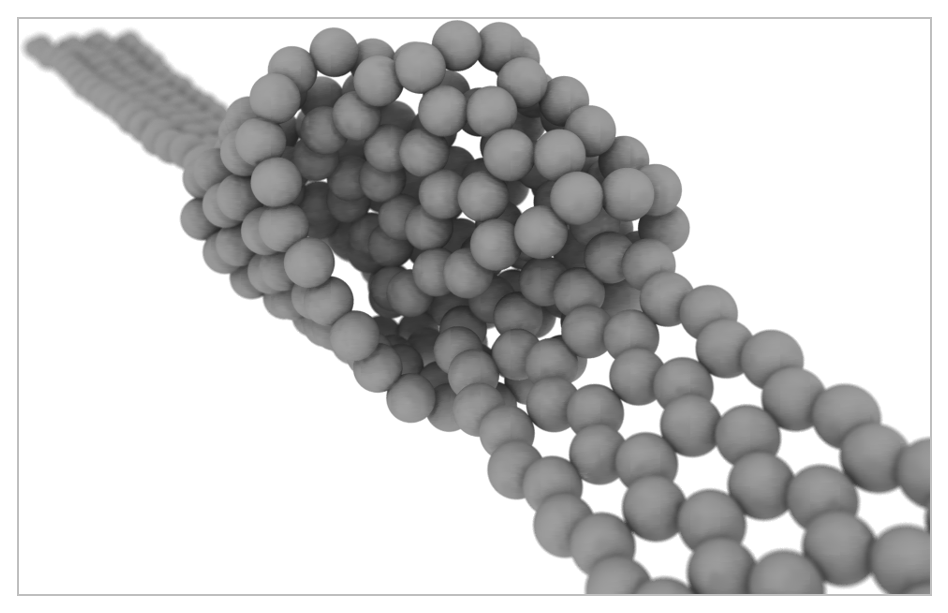
\includegraphics[width=0.48\textwidth]{images/structure}
  \caption{\label{fig:structure}  (color online) The perspective view of a graphene knot}
\end{figure}
A periodic boundary condition is applied in the y (transverse) direction, and a free boundary condition is applied in the other two directions. For each realization, all the atoms are initially placed at their equilibrium positions and then minimized at zero pressure. Then, the most two ends are fixed to reduce the drift and rotation, and the unfixed part has a random velocity according to Gaussian distribution which are then equilibrated at a given temperature 300K with a Nose-Hover thermostat3 of $2 \times10^5$ steps (0.1ns). After that, the temperature difference is built using two Nose-Hoover heat bath of 290K and 310K respectively at the two region behind the fixed region while the main parts remain NVE for another $1 \times10^7$ steps (5.0 ns) to drive the system to a stable temperature and heat flux distribution. After that, thermal conductivity is calculated according to Eq. (1). The final result is averaged over 5 realizations with different initial conditions.

The structures are prepared using interactive molecular dynamics (IMD). A graphene ribbon is mapped isodistantly to part of the knot curve described by the Trefoil equation

\begin{equation}
  \begin{aligned}
    x & = s(sin t+2 sin 2t) \\
    y & = s(cos t-2 cos 2t) \\
    z & = s(-sin 3t)
  \end{aligned}
\end{equation}

We choose s large enough to avoid oversuppesing according to the length and width of the ribbon. The structures are shown in Fig. \ref{fig:structure}



Then the system is given an initial velocity distribution of guassian at 300K while two strains are applied at the two ends towards the opposite directions. Meanwhile the mass center drifting is removed. We apply Verlet algorithm for 200000 steps when the system is in a stable state.
\begin{figure}[b]
  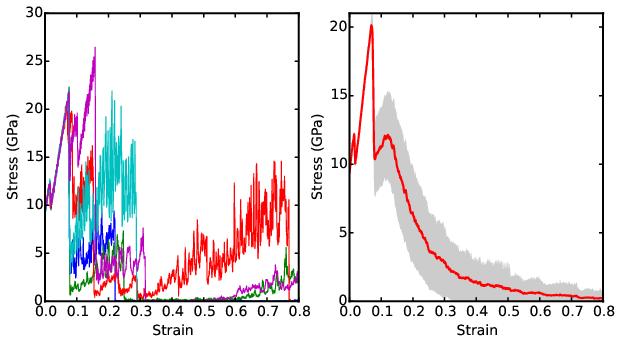
\includegraphics[width=0.48\textwidth]{images/stress}
  \caption{\label{fig:stress}  (color online) The Stres-Strain curve from 0 to a very large strain where the structures break. a) Several simulations of different random seed for MD initialization. b) The average Stress-strain curve calculated with 200 seeds. The standard error is also shown as grey ribbon.}
\end{figure}
\section{RESULTS AND DISCCUSION}

Before transport study, we have to access knowledge about the strain effect on the knot. The right end of the system is moved along x direction by a very slow velocity to apply accumulate strain ( $0.01 \angstrom / ps$ ) ,just the same operation in experiment. The stress is calculated with Vitual Therom and averaged in every 1000 steps. Fig.\ref{fig:stress} shows the break test of the knot. Under strain of 7\% the system is in it's unique stable state and it's unrelated to the initial seed. The remained stress at strain=0 is needed to prevent  the knot from release. At about 2\% there's a sudden small drop origin from bond reconstruction. At 7\% the knot break. But the knot doesn't break down, but results in another structure with inreversibility. All of the samples don't break down here. After a constant increasement of the strain the stress presents increasing fluctuate which is due to the soften of the structure which make it inconverge within the average steps. Some of the samples doesn't break even until the total stress exceed the first break critical stress. Some of them break down, but some of them keep connected but present a one-atom chain state. Between every breaks the stress-strain curve presents nearly linear and certain Young's modules.
The breaking happens at the entrance of the knot.
It's reasonable to study the properties only under stain of 5\%.
Knots ensemble shows a plastic future while graphene break very certainly.


To have a global vision of the break process we carried out more analysis on the break data as shown in Fig.\ref{fig:drop}. From figure Fig.\ref{fig:drop}a we found that the first drop happens at around 7\%  and the distribution is pretty concentrate. While the second break happens when the strain is bwteen 10\% to 40\% and is obviously broaded. This state is unstable and could be either break right after the first break or hold for a large range of strain. The 3rd and 4th breaks happens almost at the same range and has a wider range.The Young's modules distribution of the states between all the break is shown in Fig.\ref{fig:drop}b. The value at aboutn $220GPa/m$ present for the modules of unbreak knot and this value is much smaller than that of graphene ribbon of $900GPa/m$. The rest of the modules exhibit a slow decrease from 0 to $300GPa/m$ and most of them are below  $150GPa/m$ ,which shows that the system is softer.Fig.\ref{fig:drop}c shows the probobility of total break times when considering strain in range 0 to 1.0. The distribution exhibit a long tail.  Most of the samples break down within two or three times while that of four to five also have relative big probability. In the extreme situation the system could break up to 9 times. Fig.\ref{fig:drop}d shows the the probability of break down. Below 0.07 there's no probability of breaking down and the structure is stable. when above 0.07 there's about 2\% samples break down. With the strain increase the system has larger probability to break down, however the probability increase slower and slower which is due to the softer feature of the filament and the same strain contributes lesser
stress so the lesser probability of break down. When the strain reaches about 0.9 all the samples must have broken down.

\begin{figure}[b]
  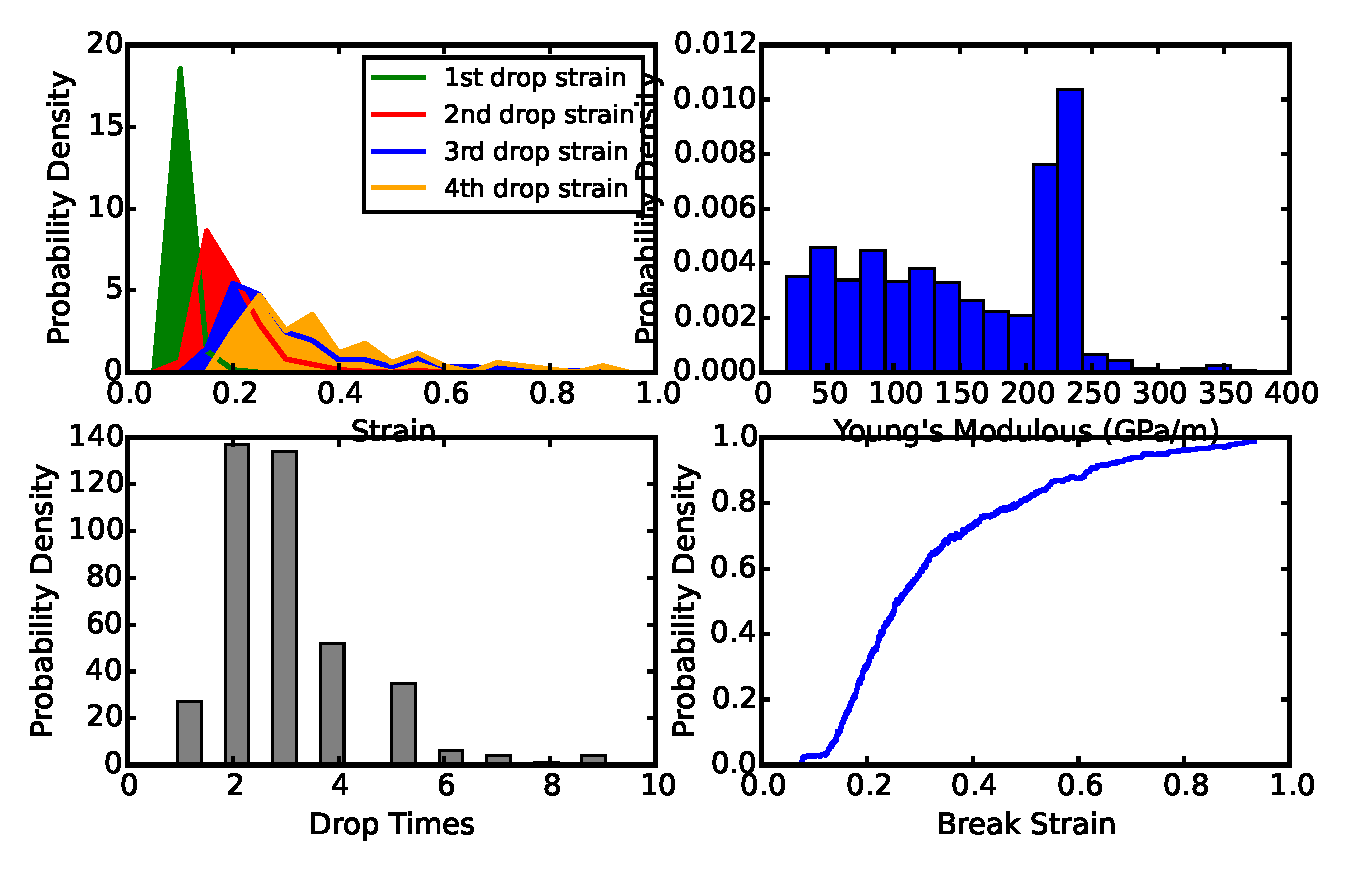
\includegraphics[width=0.48\textwidth]{images/drop}
  \caption{\label{fig:drop}  (color online) break properties statistics. a) The strain distribution of the first ,second drop and so on. b) The Young's modules distribution of the system between breaks. c) The total break times distrubution. d) The distribution of strain when the system is completely breaks}
\end{figure}


Knots posseces a hysteresis loop in its stress-strain curve. Fig.\ref{fig:cycle}a shows the cycle strain test of knot and graphene. The cycle is right hand which start from 0 and move forword to 5\% and then cycle. The drop at 2\% could not be reproduced at in the  reverse direction ,however is reproducable after the entire loop. In the reverse direction process there's also two bond reconstruction and the stress increase suddenly. But it's certain that all the sudden drop make the larger strain side the larger stress. At the minimum strain the stress still presents a positive value which means the drog is unignorable. Most test have shown that a knot without external stress will release spontaneously. Similar to that of the magnetic hysteresis loop the area enclosed by the loop equals to the work applied by the external force within one loop. The work is all converted to heat engergy and disspate by the constant temperature condition.
As a comparison,  Fig.\ref{fig:cycle}a shows the cycle of graphene which shows no hysteresis loop and the stress is not history related.

\begin{figure}[b]
  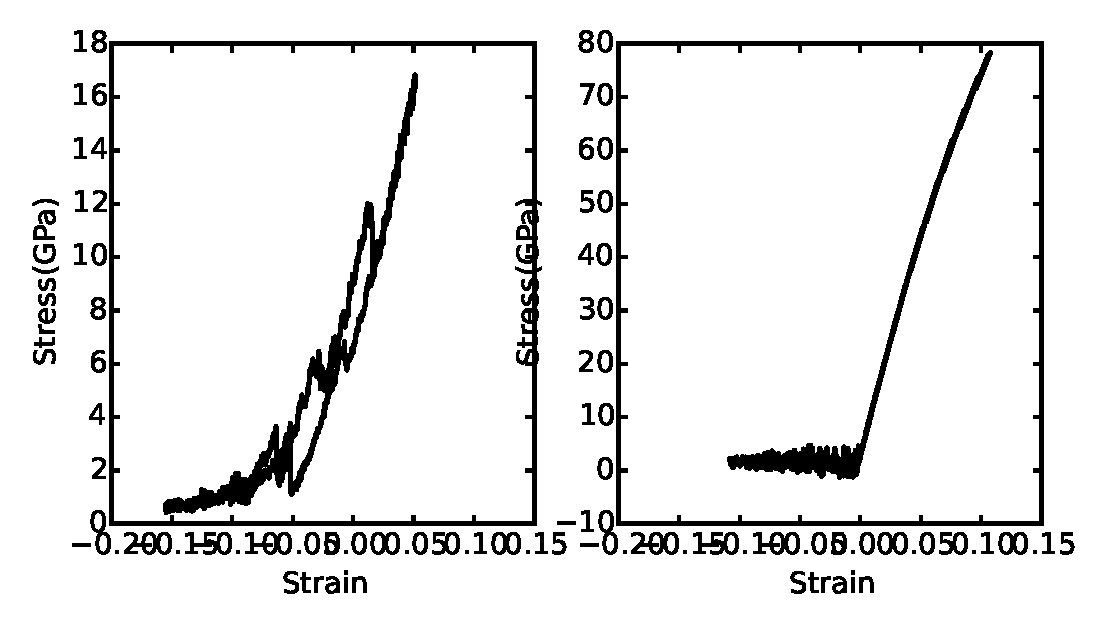
\includegraphics[width=0.48\textwidth]{images/cycle}
  \caption{\label{fig:cycle}  (color online) The Stree-Strain curve of a cycle process, where strain change slowly from 0 to max and then reduce from max to min and then back to 0. After every change 1000 steps NVT simulation is used to statistic the average stress. a) The curve for knot. b) The curve for graphene nano ribbin.}
\end{figure}

Graphene exhibit excellent transport properties but the present of knot defect will largely reduce the value and it's unknown whether the stress affects the thermal transportation properties. Fig.\ref{fig:tc_lx} shows the
thermal conductivity versus strain of different length. The strain have ignorable influence on the thermal condcutivity. However the strain effect of graphene is very clear. This is because the strain is eliminated by the out-of-plane displacement which has little influence on the in-plane bond length.
\begin{figure}[b]
  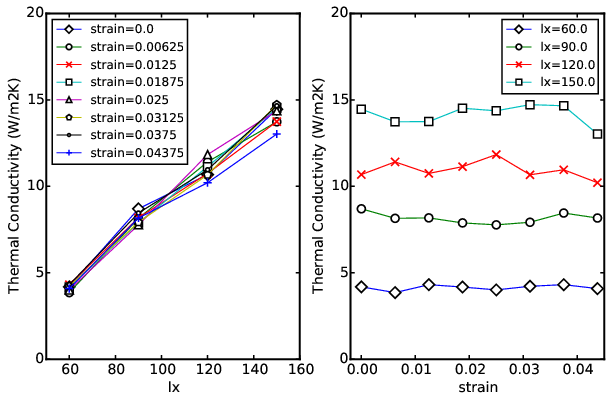
\includegraphics[width=0.48\textwidth]{images/tc_lx}
  \caption{\label{fig:tc_lx}  (color online) The perspective view of a graphene knot}
\end{figure}

At a large scale the knot superlattice could be regard as a particle-spring chain and we also studyed the thermal conductivity of the knot superlattice.
The TC of interface is  called Kapitza conductance and is shown in Fig.\ref{fig:tc_nx}a. TC increase with nx linearly and doesn't converge in the computational effort.Fig.\ref{fig:tc_nx}d shows the temperature profile of different nx. The position is normilzed to 1.0.With the increase of nx the profile converge to linear and the detail of the knot is no more important.
The total temperature drop at the knots are shown in Fig.\ref{fig:tc_nx}c. The total temperature drop increase when the number of knots increases because the temperature load on each of the ribbon decrease and the real temperature drop all concentrate on the knots. The average temperature drop of every knot is shown in Fig.\ref{fig:tc_nx}b. When nx is small dT is very large and with the increase of nx this value decrease a lot. This is obvious becasue the total temperature is constant but the number of knot increases.

\begin{figure}[b]
  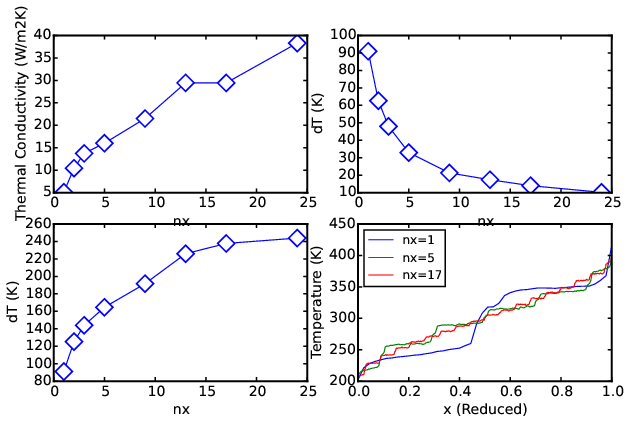
\includegraphics[width=0.48\textwidth]{images/tc_nx}
  \caption{\label{fig:tc_nx}  (color online) The position is normilzed to 1.0 }
\end{figure}

For a deeper understanding of the transport properties we calculate the phonon density of states of graphene nanoribbon,the knot region and the bulk rigion of the knot. The bulk rigion is far away from the knot and has the same structure with the GNR. However the DOS of bulk regioin is not like graphene but silimar to the knot region. This suggests that the present of the knot import a non-local influence to the structure.

\begin{figure}[b]
  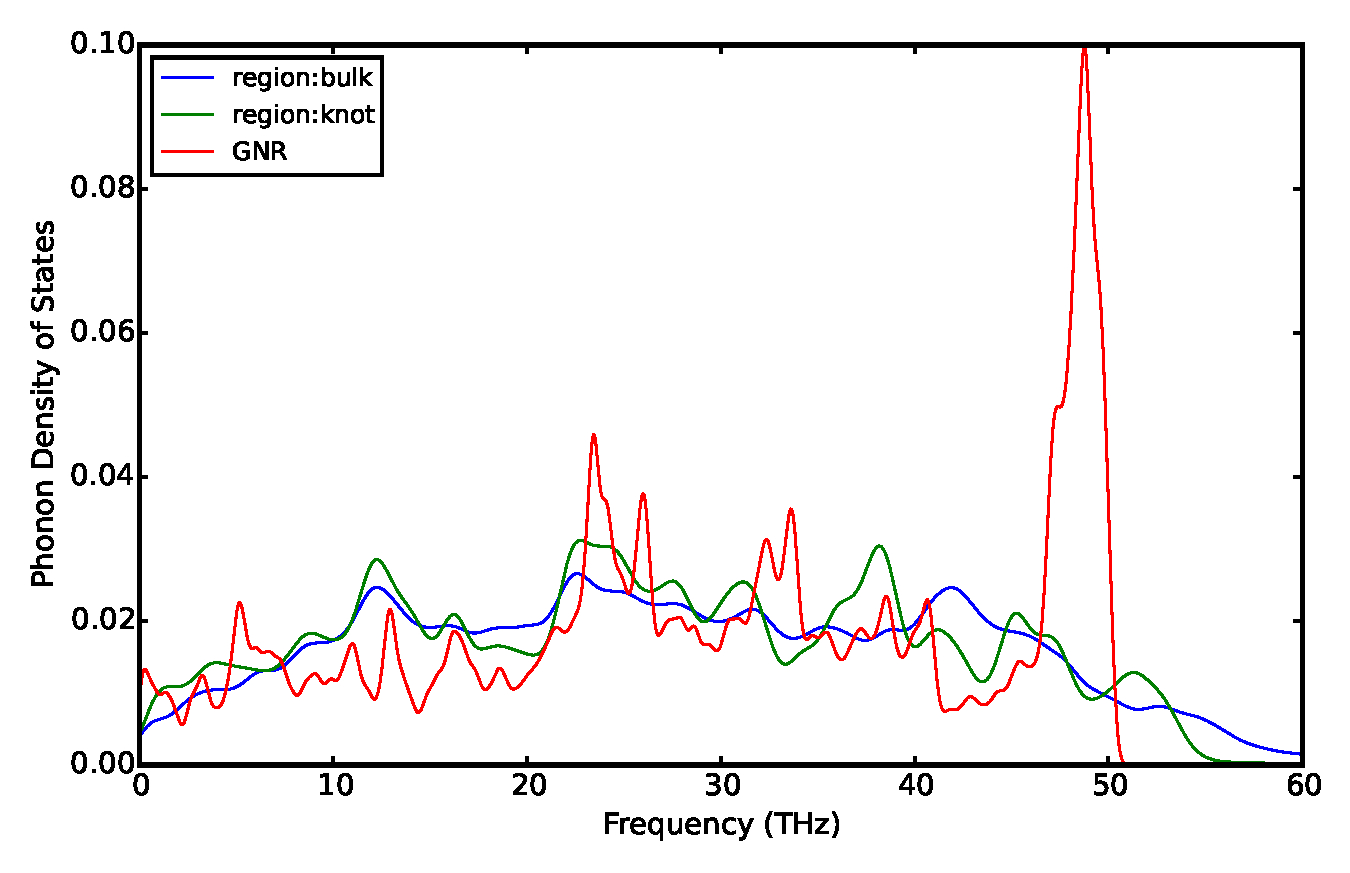
\includegraphics[width=0.48\textwidth]{images/dos}
  \caption{\label{fig:dos}  (color online) The position is normilzed to 1.0 }
\end{figure}

\section{CONCLUSIONS}
In this paper we simulated the mechanical properties and  thermal transport properties of graphene nano knot with nonequilibrium molecular dynamics(NEMD).

\quad \\
\section{ACKNOWLEGEMENTS}
This paper was partially supported by the National Natural Science Foundation of China, the Special Funds for Major State Basic Research, the Foundation for the Author of National Excellent Doctoral Dissertation of China, the Program for Professor of Special Appointment at Shanghai Institutions of Higher Learning, and the Research Program of Shanghai Municipality and the Ministry of Education.


\bibliography{ref}
\end{document}